

\newpage
\section{11-02-2019: ITERATORI E GENERICS}
\noindent \textbf{ITERATORE e ITERABLE}\newline
\textbullet\  \textit{Iteratore}: E' un pattern, uno stile di programmazione. Il pattern degli iteratori esiste in tutti i linguaggi ad oggetti. Con iteratore intendiamo lo scorrimento di una collezione di elementi. L'iteratore serve quindi a scorrere una collection.\newline
\textbullet\ \textit{Iterable}: E' una super interfaccia, e l'interfaccia \textit{Collection} implementa questa super interfaccia. Iterable è super tipo di tutte le interfacce.

\noindent Se una interfaccia rappresenta una super interfaccia significa che non ha un genitore, anche se in realtà estende \textit{Object}


\noindent \textbf{MAPPA}\newline
Una mappa è una struttura dati che mappa chiavi e valori, ha quindi due parametri: il tipo della chiave e il tipo del valore. Una mappa è una \textit{collection} solo se vista come una collection di coppie. Infatti una \textit{collection} è figlia di \textit{iterable} (la posizione più alta nella gerarchia), ma una \textit{mappa} NON è figlia di \textit{iterable}
\begin{center}
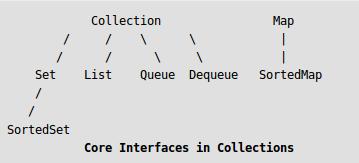
\includegraphics[width=%
0.6\textwidth]{MapInterface}
\end{center} 

\noindent \textbf{SOTTO TIPI}\newline
Ci riferiamo ad un oggetto usando la parola \textit{sottotipo} quando esso è:\newline
\textbullet\ O una sottoclasse (extends) \newline
\textbullet\ O una sotto interfaccia (implements) \newline
Ad esempio ArrayList ha come superclasse abstract arrayList. ArrayList implementa collection. Quindi ne è sottotipo ma non sottoclasse.

\noindent \textbf{GENERICS}\newline
<? extends classe> e <? extends E> rappresentano un tipo. \newline
La \textit{SUBSUMPTION} non funziona in genere sempre tra GENERICS. Per il parametro stesso c'è subsumption, ma non per le collection. Il tipo con il ? accetta sottotipi di parametri.\newline
\textbullet\ Il TIPO ESTERNO gode sempre della subsumption.(List<Int>: List è tipo esterno)
\begin{lstlisting}[basicstyle=\small,]
 ArrayList<Int> è sottotipo di List<Int>
\end{lstlisting}
\noindent \textbullet\ Il TIPO INTERNO non gode mai della subsumption(cioè il tipo all'interno di <>). La subsumption si può fare solo usando i generics( quindi con <? extends E>)
\begin{lstlisting}[basicstyle=\small,]
 ArrayList<Iterable> non è sottotipo di ArrayList<Collection>
\end{lstlisting}
\noindent Si dice che abbiamo quindi "\textit{Invarianza del subtyping}": se ciò non fosse le subsumption funzionerebbero anche nel tipo interno e questo rischierebbe la totale spaccatura del linguaggio (senza l'invarianza si possono creare problemi di cast ed oggetti).\newline
Se cosi non fosse in java non verrebbero mai rispettate le regole delle classi.
\begin{lstlisting}[basicstyle=\small,]
/* Illegal code - because otherwise life would be Bad */
List<Dog> dogs = new ArrayList<Dog>(); /* ArrayList implements List */
List<Animal> animals = dogs; /*  Awooga awooga */
animals.add(new Cat());
Dog dog = dogs.get(0); /* This should be safe, right? */
\end{lstlisting}

\noindent Java di unico ha che esiste il wildchart (?), che è un modo controllato per risolvere il problema della subsumption dei tipi interni. \newline
Prima dei generics (2003/2004) in java si programmava tutto a typecast. Per motivi di retrocompatibilità è possibile programmare in tutti e due i modi. E' comunque consigliato usare la programmazione con i \textit{generics}. \newline
Metodi che ritornano un booleano iniziano con sempre come se fossero domande; es: hasNext, isEmpty etc.. \newline
Un iteratore non può essere costruito con un new perchè è un'interfaccia. 
\newpage
